%===================================== CHAP 4 =================================

\chapter{Technology}
% ========================== section ============================
\section{Framework - Theano}

Theano is a python library which is able to compile the code both to C and to CUDA, thus enabling running the code on a GPU. This is a much more efficient approach today when running ANNs, as they may run fairly decentralized, using a shared memory for weights. In this thesis, we will use Theano to implement the ANN model and experiments that we outline in chapter \ref{future_work}.

\subsection{A Brief Overview}

Symbolic programming.
\\
Theano operates on symbolic constructs, called tensors; general mathematical constructs. Theano constructs a graph of the provided symbolic definitions. Allowomg for symbolic differentiation and manipulation through a syntactic and semantic analysis of the code, as well as optimalization. The compiler optimizes the code, before compiling it according to the provided environmental parameters. Leading to a higly optimized C or CUDA implementation and execution of the symbolically defined code.
Note, however, that this renders debugging somewhat harder, as the executable code will be quite different from what is written in Python/Theano. Thus the programmer may need to predict how the code will be compiled, making it highly recommendable, if not even necessary, to have some previous knowledge within C and/or how the Python-library's compilation process works.

\begin{figure}
\centering
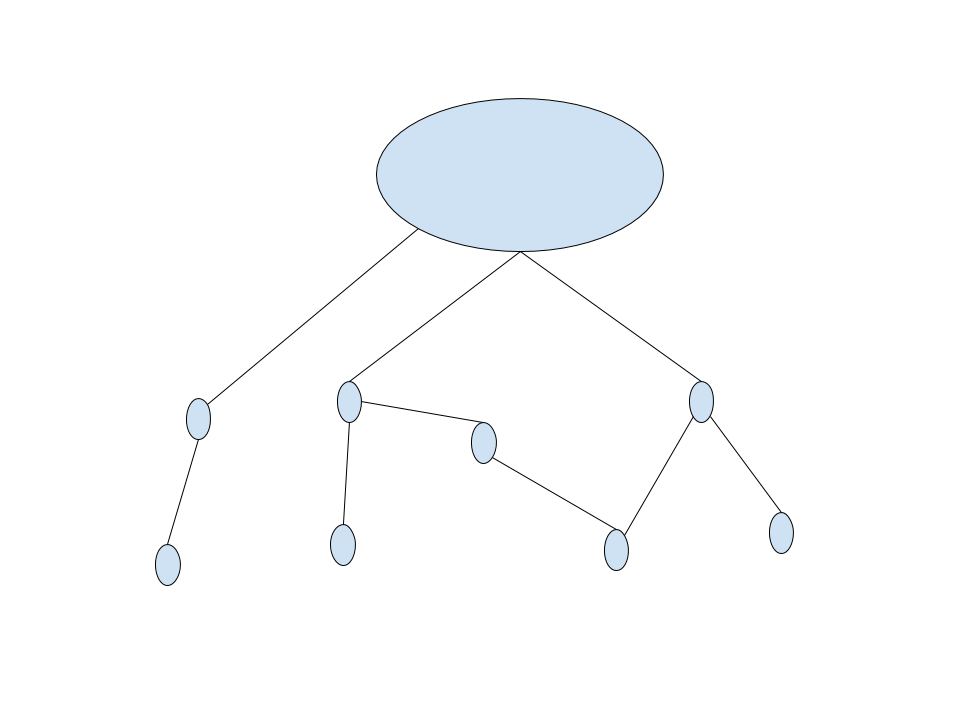
\includegraphics[width=10cm]{fig/dummy_theano_graph}
\caption{Graph manipulation of tensors in Theano during the compilation process.}
\label{fig:graph_manipulation_theano}
\end{figure}

\subsection{Setup}

In order to use Theano, certain dependencies need to be setup. These are fairly straightforward when it comes to compiling to C-code. However, when using the GPU-flag to compile the Theano/Python code to CUDA, the process becomes less straightforward. In order to do so, certain libraries need to be installed, such as for compiling to CUDA. Furthermore, system dependencies need to be setup, and drivers installed. In this thesis and preliminary study, we setup Theano for use with a GPU on a system with an NVIDIA card, using Ubuntu 14.04 LTS. Furthermore, we used the guide found on \\http://deeplearning.net/software/theano/install.html\#install to obtain installation instructions for doing so.

% ========================== section ============================
\section{GPU Optimization}

\subsection{The Parallelism of ANNs}

Theoretical complete decentralization, rendering ANNs completely parallelizable. This may in practice be achieved using a smart implementation for a single network. Decentralization becomes slightly more complex when introducing dual-networks, due to certain criteria for when to run, which may have to pass control back to the interpreter, i.e. when non-Theano-library code has to run. Therefore, possible techniques for running the networks asynchronously should be investigated, which may tremendously improve (reduce) the execution time of the experimental model.

\subsection{A Hardware Example}
A modern chip of these days may contain a thousand CUDA cores, each running at over a thousand MHz. As an example, we have compared one of the cheap high-end GPUs such as NVIDIAs GeForce GTX 960 with an i7 CPU running at about 3.2 GHz in a simplified manner.
\\
The GTX 960 has 1024 CUDA cores, each running at a frequency of 1127 MHz (base).

For the trivial case where the algorithm is entirely decentralized, we have that it could perform,

\begin{center}
\begin{math}
    1024 * 1127 = 1 154 048 * 10^6 \text{ operations per second},
\end{math}
\end{center}
whereas the CPU performs about $3.2 * 10^9$ operations per second.
Theoretically making the GPU $\frac{1154048*10^6}{3.2*10^9} = 360.640$ times more efficient.
\\
Now, the crucial point here to note is that using the GPU requires a substantial amount of overhead in order to transfer instructions and data to on-chip memory. Furthermore, the results need to be transferred back into RAM. It is also important to note that if control has to be passed back to the interpreter during run-time execution of a program in Python/Theano, information on the GPU has to be transferred back to memory, before the CPU may continue to perform the required operations, optionally returning 'control' back to the GPU again. This makes the BUS size a possible bottleneck for run-time efficiency, and does in either way introduce a significant time delay for data-bus-transfer during run-time.

Nevertheless, in the best-case scenario, it is only the setup of the algorithm on the GPU and returning the results which will cause bus-traffic. Rendering the few seconds such overhead takes negligible for algorithms which may spend hours executing solely on the CPU. In such a scenario, we may in theory spend an hour doing crunching an algorithm on the CPU, whilst the GPU may execute it in only about ten seconds. This is without the few seconds spent on overhead before and after execution. Note that a few seconds also have to be added in to such an estimation for every time the interpreter needs control over the program. We will not go in depth into such calculations here, as the complexity of the temporal dependencies in the hardware is outside the scope of this thesis. However, we hope that the former simplified example may provide the reader with a gist of the potential performance boost that may be gained by using GPUs and Theano for training ANNs.

Concluding, parallelizing algorithms for running on GPUs may with average modern high-end GPUs lead to a potentially dramatic decrease in execution time for highly parallelizable algorithms.

% ========================== section ============================
\section{A Preliminary Implementation}

We tested a simple ANN in Theano, more specifically by using a traditional FFBP ANN, based on the implementation of
\\(http://nbviewer.ipython.org/github/craffel/theano-tutorial/blob/master/Theano\%20Tutori
\\al.ipynb), in order to test the Theano library as well as our local installation. Note that the author calls it a multi-layer perceptron, as the term has been loosened to encompass all types of artificial neurons in recent years. It is, in either way, a multi-layer ANN, whose units employ the sigmoidal transfer function. In the following example, the data set is classified into two clusters, rendering the resulting classification binary this could easily be extended, however, by increasing the dimensionality of the output layer.


Following is a code snippet from the implementation (for the full code please visit the link above):

\begin{verbatim}
# Create Theano variables for the MLP input
mlp_input = T.matrix('mlp_input')
# ... and the desired output
mlp_target = T.vector('mlp_target')

# Create a function for computing the cost of the network 
# given an input
cost = mlp.squared_error(mlp_input, mlp_target)
# Create a theano function for training the network
train = theano.function([mlp_input, mlp_target], cost,
                updates=gradient_updates_momentum(cost,
                mlp.params, learning_rate, momentum))
# Create a theano function for computing the MLP's output 
# given some input
mlp_output = theano.function([mlp_input], mlp.output(mlp_input))
\end{verbatim}

Theano symbolic function definition. Theano infers function and compiles the corresponding C/CUDA-code. See table below for the average results of a few runs of the implemented algorithm.
\\\\
MLP details:
\\
Simply a binary FFBP ANN as elaborated on in chapter \ref{BP}.
\\
Input data: N two-dimensional points (x, y). Gaussian distribution.
\\\\
ANN:
\\
2-4-1 ANN.
\\
Fully connected between the layers.
\\
So what happens is: 
\\
For every data point: 
FF.
\\
Calculate SE.
\\
Calculate gradient for minimizing the SE.
\\
Update weight matrix using BP.
\\\\
The result:
\\
A FFBP ANN that is in a local minima for the SSE, i.e. it has extracted two means which minimizes the error criterion, effectively creating two clusters.


\begin{table}
\begin{center}
    \begin{tabular}{ | l | l | l | l |}
    \hline
    \textbf{Measure (seconds)} & \textbf{GPU} & \textbf{CPU} \\ \hline
     Setup, $N=10 000$ & $\approx0.8$ & $\approx7.0$ \\ \hline
     Training, 1k iterations &  $\approx1.5$ & $\approx9.0$ \\ \hline
     Training, 10k iterations &  $\approx14.6$ & $\approx65.8$ \\ \hline
    \end{tabular}
\end{center}
\caption{Presenting the results from running the MLP as elaborated on above on two data-sets consisting of $N=10 000$ two-dimensional data points, training for $1000$ and $10 000$ iterations. Note that the execution time was about 4-6 times faster when running on a GPU, and this is for a non-optimized version of the algorithm. See figure \ref{fig:theano_mlp_demo} for a plot of the results.}
\label{tab:MLP_gpu_vs_cpu}
\end{table}

The results of \ref{tab:MLP_gpu_vs_cpu} are as expected, as we cannot given the architecture of the ANN achieve a performance increase which is greater than the relative number of neurons in the network. The factor of increase relative to the number of neurons does obviously depend on the algorithm and implementation. The performance increase of this implementation suggests that the implementation is fairly optimal given the network size and performance gain for using the GPU.

\begin{figure}
\centering
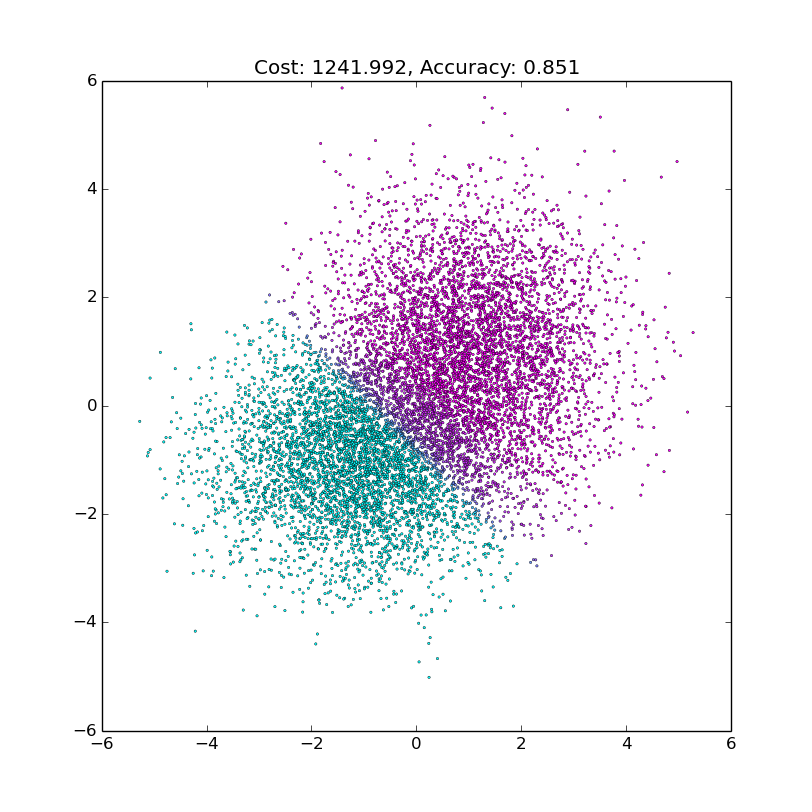
\includegraphics[width=12cm]{fig/MLP_cluster_N_10000_1kiter}
\caption{Illustrating the final plot after training for $10 000$ iterations on a data set with $N=10 000$ normally distributed two-dimensional data points. The cost is the sum of squared errors of the Euclidean distance between the predicted data points and the actual data points, and the accuracy is the relative frequency of correctly classified data points. Note the blue line between the two clusters, which results from data points being classified into the two different classes on top of each other, resulting into blue when the colours blend. This line is in fact representing the separating hyperplane (linear separator in this case).}
\label{fig:theano_mlp_demo}
\end{figure}

In this implementation, BP is performed layer-wise, actually taking into account the current gradient when using the chain-rule for back-propagation of the error signal throughout the network. However;
Because of the algorithmic implications of convergence being guaranteed for using the gradients of former time-steps, the algorithm will also be tolerant towards aliasing of the shared memory of weights!
This actually means that the algorithm could be optimized in terms of using former error-gradients when calculating the updates. Note however, that this may increase the number of iterations required for a satisfactory accuracy, particularly in the case of attempting to segment randomly distributed data.

% ========================== section ============================
\section{Notes}

Should include some algorithmic details related to the equations of chpt. 3? Could optionally just write this in chpt. 4, and move it to chpt. 3 if Keith finds it more suitable.

Should test whether overwriting a matrix element through borrowing in Theano overwrites the entire matrix or only the matrix element. The former would be unacceptable.


\cleardoublepage